\setcounter{definition}{0} \setcounter{property}{0} \setcounter{claim}{0} \setcounter{fact}{0} \setcounter{corollary}{0} \setcounter{figure}{0}
\section{Why DP Table? Why not Recursive Programming?}

In all the DP algorithms we've designed, we always use a table to store
the optimal solution of subproblems; when solving larger
subproblems, we simply query the table and fetch the optimal
solutions as needed. 
This leads to a bottom-up strategy, i.e., we start from solving
smaller subproblems as they will be needed by larger ones.
Is this strategy always necessary?
Can we directly solve the original problem with recursive programming?

Let's try.
Consider the edit distance problem~(Lecture 26).
The DP algorithm we designed there uses the recursion below.
\begin{displaymath}
F(i,j) = \min\left\{
	\begin{array}{llll}
	F(i-1,j-1) + \delta(X[i] \neq Y[j]) \\
	F(i-1,j) + 1 \\
	F(i,j-1) + 1 \\
	\end{array}
\right.
\end{displaymath}

We write a recursive procedure: define $F(i,j)$
returns the edit distance between $X[1\cdots i]$ and $Y[1\cdots j]$.

\begin{minipage}{0.8\textwidth}
	\aaA {7}{function $F(i,j)$}\xxx
	\aab {if $i = 0$: return $j$;}\xxx
	\aab {if $j = 0$: return $i$;}\xxx
	\aab {$z_1 = F(i-1,j-1) + \delta(X[i] \neq Y[j])$;}\xxx
	\aab {$z_2 = F(i-1,j) + 1$;}\xxx
	\aab {$z_3 = F(i,j-1) + 1$;}\xxx
	\aab {return $\min\{z_1,z_2,z_3\}$;}\xxx
	\aaa {end function;}\xxx
\end{minipage}

We then call $F(m,n)$, where $m=|X|$ and $n=|Y|$.
This is a correct algorithm.
How about its running time?
We define $T(m,n)$ as the running time of $F(m,n)$.
We have $T(m,n) = T(m-1,n-1) + T(m-1,n) + T(m,n-1) + 1$.
To \emph{approximate} $T(m,n)$, assume that $m=n$.
Notice also that $T(m-1,n) \ge T(m-1,n-1)$
and $T(m,n-1) \ge T(m-1,n-1)$.
We can write $T(n,n) \ge 3T(n-1,n-1) + 1$.
Hence, $T(n,n) \ge \Theta(3^n)$.
So, above algorithm runs in exponential-time!
This suggests that recursive procedure is a bad strategy.

\begin{figure}[b]
\centering{\tikzset{every picture/.style={line width=0.75pt}} %set default line width to 0.75pt        

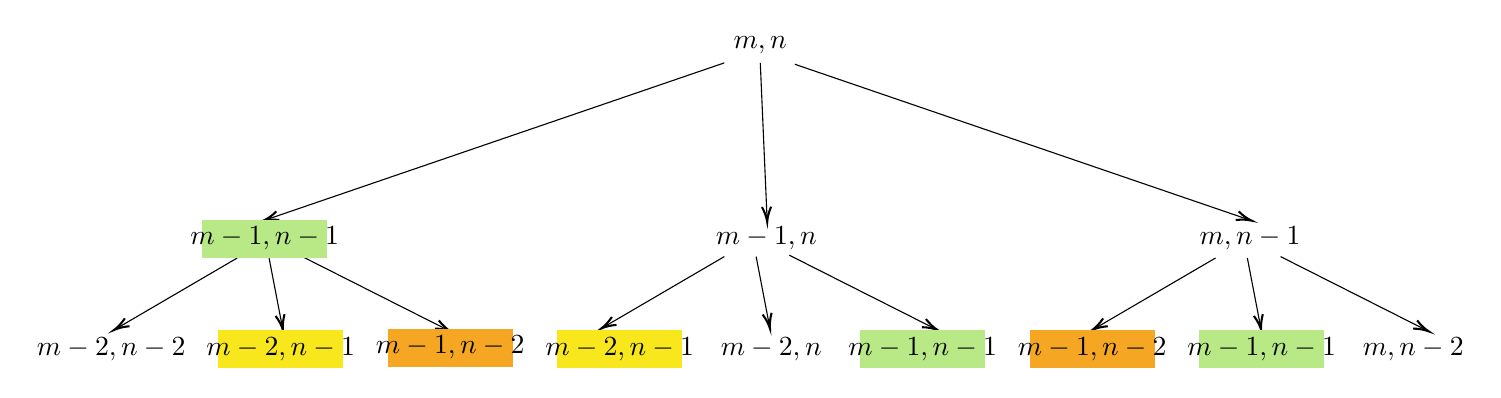
\begin{tikzpicture}[x=0.5pt,y=0.5pt,yscale=-1,xscale=1]
%uncomment if require: \path (0,284); %set diagram left start at 0, and has height of 284

%Straight Lines [id:da1383331413383435] 
\draw    (522.5,36) -- (191.39,149.35) ;
\draw [shift={(189.5,150)}, rotate = 341.1] [color={rgb, 255:red, 0; green, 0; blue, 0 }  ][line width=0.75]    (10.93,-3.29) .. controls (6.95,-1.4) and (3.31,-0.3) .. (0,0) .. controls (3.31,0.3) and (6.95,1.4) .. (10.93,3.29)   ;
%Straight Lines [id:da715204982720897] 
\draw    (548.5,36) -- (553.41,149) ;
\draw [shift={(553.5,151)}, rotate = 267.51] [color={rgb, 255:red, 0; green, 0; blue, 0 }  ][line width=0.75]    (10.93,-3.29) .. controls (6.95,-1.4) and (3.31,-0.3) .. (0,0) .. controls (3.31,0.3) and (6.95,1.4) .. (10.93,3.29)   ;
%Straight Lines [id:da8831806389031782] 
\draw    (573.5,37) -- (901.61,149.35) ;
\draw [shift={(903.5,150)}, rotate = 198.9] [color={rgb, 255:red, 0; green, 0; blue, 0 }  ][line width=0.75]    (10.93,-3.29) .. controls (6.95,-1.4) and (3.31,-0.3) .. (0,0) .. controls (3.31,0.3) and (6.95,1.4) .. (10.93,3.29)   ;
%Straight Lines [id:da6762777724306107] 
\draw    (170.5,177) -- (83.23,227.99) ;
\draw [shift={(81.5,229)}, rotate = 329.7] [color={rgb, 255:red, 0; green, 0; blue, 0 }  ][line width=0.75]    (10.93,-3.29) .. controls (6.95,-1.4) and (3.31,-0.3) .. (0,0) .. controls (3.31,0.3) and (6.95,1.4) .. (10.93,3.29)   ;
%Straight Lines [id:da9537842571445845] 
\draw    (193.5,177) -- (203.12,227.04) ;
\draw [shift={(203.5,229)}, rotate = 259.11] [color={rgb, 255:red, 0; green, 0; blue, 0 }  ][line width=0.75]    (10.93,-3.29) .. controls (6.95,-1.4) and (3.31,-0.3) .. (0,0) .. controls (3.31,0.3) and (6.95,1.4) .. (10.93,3.29)   ;
%Straight Lines [id:da25240177172893863] 
\draw    (217.5,176) -- (322.71,229.1) ;
\draw [shift={(324.5,230)}, rotate = 206.78] [color={rgb, 255:red, 0; green, 0; blue, 0 }  ][line width=0.75]    (10.93,-3.29) .. controls (6.95,-1.4) and (3.31,-0.3) .. (0,0) .. controls (3.31,0.3) and (6.95,1.4) .. (10.93,3.29)   ;
%Straight Lines [id:da4227912867383341] 
\draw    (522.5,176) -- (435.23,226.99) ;
\draw [shift={(433.5,228)}, rotate = 329.7] [color={rgb, 255:red, 0; green, 0; blue, 0 }  ][line width=0.75]    (10.93,-3.29) .. controls (6.95,-1.4) and (3.31,-0.3) .. (0,0) .. controls (3.31,0.3) and (6.95,1.4) .. (10.93,3.29)   ;
%Straight Lines [id:da490335830545392] 
\draw    (545.5,176) -- (555.12,226.04) ;
\draw [shift={(555.5,228)}, rotate = 259.11] [color={rgb, 255:red, 0; green, 0; blue, 0 }  ][line width=0.75]    (10.93,-3.29) .. controls (6.95,-1.4) and (3.31,-0.3) .. (0,0) .. controls (3.31,0.3) and (6.95,1.4) .. (10.93,3.29)   ;
%Straight Lines [id:da44453803269503656] 
\draw    (569.5,175) -- (674.71,228.1) ;
\draw [shift={(676.5,229)}, rotate = 206.78] [color={rgb, 255:red, 0; green, 0; blue, 0 }  ][line width=0.75]    (10.93,-3.29) .. controls (6.95,-1.4) and (3.31,-0.3) .. (0,0) .. controls (3.31,0.3) and (6.95,1.4) .. (10.93,3.29)   ;
%Straight Lines [id:da6159232694423369] 
\draw    (877.5,177) -- (790.23,227.99) ;
\draw [shift={(788.5,229)}, rotate = 329.7] [color={rgb, 255:red, 0; green, 0; blue, 0 }  ][line width=0.75]    (10.93,-3.29) .. controls (6.95,-1.4) and (3.31,-0.3) .. (0,0) .. controls (3.31,0.3) and (6.95,1.4) .. (10.93,3.29)   ;
%Straight Lines [id:da04820263440719896] 
\draw    (900.5,177) -- (910.12,227.04) ;
\draw [shift={(910.5,229)}, rotate = 259.11] [color={rgb, 255:red, 0; green, 0; blue, 0 }  ][line width=0.75]    (10.93,-3.29) .. controls (6.95,-1.4) and (3.31,-0.3) .. (0,0) .. controls (3.31,0.3) and (6.95,1.4) .. (10.93,3.29)   ;
%Straight Lines [id:da4987937509957987] 
\draw    (924.5,176) -- (1029.71,229.1) ;
\draw [shift={(1031.5,230)}, rotate = 206.78] [color={rgb, 255:red, 0; green, 0; blue, 0 }  ][line width=0.75]    (10.93,-3.29) .. controls (6.95,-1.4) and (3.31,-0.3) .. (0,0) .. controls (3.31,0.3) and (6.95,1.4) .. (10.93,3.29)   ;

% Text Node
\draw (548.38,23.47) node   [align=left] {$\displaystyle m,n$};
% Text Node
\draw  [color={rgb, 255:red, 184; green, 233; blue, 134 }  ,draw opacity=1 ][fill={rgb, 255:red, 184; green, 233; blue, 134 }  ,fill opacity=1 ][line width=0.75]   (145.88,149.97) -- (234.88,149.97) -- (234.88,175.97) -- (145.88,175.97) -- cycle  ;
\draw (190.38,162.97) node   [align=left] {$\displaystyle m-1,n-1$};
% Text Node
\draw (552.88,162.97) node   [align=left] {$\displaystyle m-1,n$};
% Text Node
\draw (902.38,162.97) node   [align=left] {$\displaystyle m,n-1$};
% Text Node
\draw (79.38,242.72) node   [align=left] {$\displaystyle m-2,n-2$};
% Text Node
\draw  [color={rgb, 255:red, 248; green, 231; blue, 28 }  ,draw opacity=1 ][fill={rgb, 255:red, 248; green, 231; blue, 28 }  ,fill opacity=1 ][line width=0.75]   (157.38,229.72) -- (246.38,229.72) -- (246.38,255.72) -- (157.38,255.72) -- cycle  ;
\draw (201.88,242.72) node   [align=left] {$\displaystyle m-2,n-1$};
% Text Node
\draw  [color={rgb, 255:red, 245; green, 166; blue, 35 }  ,draw opacity=1 ][fill={rgb, 255:red, 245; green, 166; blue, 35 }  ,fill opacity=1 ][line width=0.75]   (279.88,228.72) -- (368.88,228.72) -- (368.88,254.72) -- (279.88,254.72) -- cycle  ;
\draw (324.38,241.72) node   [align=left] {$\displaystyle m-1,n-2$};
% Text Node
\draw  [color={rgb, 255:red, 248; green, 231; blue, 28 }  ,draw opacity=1 ][fill={rgb, 255:red, 248; green, 231; blue, 28 }  ,fill opacity=1 ][line width=0.75]   (402.38,229.72) -- (491.38,229.72) -- (491.38,255.72) -- (402.38,255.72) -- cycle  ;
\draw (446.88,242.72) node   [align=left] {$\displaystyle m-2,n-1$};
% Text Node
\draw (556.38,242.72) node   [align=left] {$\displaystyle m-2,n$};
% Text Node
\draw  [color={rgb, 255:red, 184; green, 233; blue, 134 }  ,draw opacity=1 ][fill={rgb, 255:red, 184; green, 233; blue, 134 }  ,fill opacity=1 ][line width=0.75]   (621.38,229.72) -- (710.38,229.72) -- (710.38,255.72) -- (621.38,255.72) -- cycle  ;
\draw (665.88,242.72) node   [align=left] {$\displaystyle m-1,n-1$};
% Text Node
\draw  [color={rgb, 255:red, 245; green, 166; blue, 35 }  ,draw opacity=1 ][fill={rgb, 255:red, 245; green, 166; blue, 35 }  ,fill opacity=1 ][line width=0.75]   (743.88,229.72) -- (832.88,229.72) -- (832.88,255.72) -- (743.88,255.72) -- cycle  ;
\draw (788.38,242.72) node   [align=left] {$\displaystyle m-1,n-2$};
% Text Node
\draw  [color={rgb, 255:red, 184; green, 233; blue, 134 }  ,draw opacity=1 ][fill={rgb, 255:red, 184; green, 233; blue, 134 }  ,fill opacity=1 ][line width=0.75]   (866.38,229.72) -- (955.38,229.72) -- (955.38,255.72) -- (866.38,255.72) -- cycle  ;
\draw (910.88,242.72) node   [align=left] {$\displaystyle m-1,n-1$};
% Text Node
\draw (1020.38,242.72) node   [align=left] {$\displaystyle m,n-2$};


\end{tikzpicture}

}
\caption{First 3 levels of the recursive tree of above procedure.
Identical recursive calls are marked with the same color.}
\label{fig:tree}
\end{figure}


Note that there are $\Theta(mn)$ distinct subproblems, i.e., $F(i,j)$, $0\le i
\le m$, $0\le j \le n$. The reason why above
algorithm runs in exponential time is that it keeps solving the \emph{same}
subproblems. See Figure~\ref{fig:tree}. This again suggests the necessity
of maintaining a table to store the optimal solutions so as to avoid
repeating resolving the same ones.
An alternative way to understand it is that, subproblems will be used
multiple times by different larger subproblems, hence it's beneficial
to store them.


Both divide-and-conquer algorithms and dynamic programming algorithm
rely on a recursive formula that reduces larger subproblems into smallers.
Why for D\&C algorithm we don't maintain a table?
There are two reasons.
First, in (most) D\&C algorithms, subproblems don't overlap~(while in DP algorithms they do, as showed in Figure~\ref{fig:tree}), or in other words,
each subproblem will be used only once. Therefore there is no difference between
solving recursively or by using a table.
Second, in (most) D\&C algorithms, the size of the subproblem is usually reduced by a \emph{fixed ratio}~(for example, $n\to n/2$),
and consequently the height of the recursive tree is $\Theta(\log n)$. 
Hence there is \emph{no need} to maintain a table, as solving all subproblems on the fly is still efficient.
On the contrary, in (most) DP algorithms, the size of the subproblem is usually reduced by a \emph{constant}~(for example, $n\to n-1$),
and consequently the height of the recursive tree is $\Theta(n)$;
solving all subproblems on the fly will require exponential-time, as we just showed.

